\chapter{Quiebre Espont'aneo de Simetr'ia y Mecanismo de Higgs}

En la naturaleza, una variedad de simetr'ias  elegantes  nos rodean. Sin embargo, tambi'en hay muchos ejemplos de simetr'ias en la naturaleza que est'an rotas. 
En casos donde esto ocurre se le denomina  \textit{quiebre espont'anea de simetr'ia}, es decir, el hamiltoniano es invariante bajo una cierta simetr'ia, pero la simetr'ia se rompe porque el estado fundamental del hamiltoniano no es invariante.  
Ejemplos  simples vienen de f'isica del estado s'olido, donde el fen'omeno de la ruptura espont'anea de  simetr'ia es bastante com'un. Consideremos un material ferromagn'etico, de manera que los 'atomos poseen un spin $\sigma_i$. Aunque el hamiltoniano no escoja una  direcci'on en  particular en el espacio, el estado fundamental de la teor'ia, sin embargo, puede consistir en 'atomos cuyos spines est'en todos alineados en la misma direcci'on. Por lo tanto, la simetr'ia de rotaci'on puede ser rota por el estado de vac'io, incluso cuando el hamiltoniano permanezca completamente sim'etrico. Para restaurar la simetr'ia, se debe calentar el material ferromagn'etico a una alta temperatura, donde los 'atomos vuelvan a estar alineados aleatoriamente.

\section{Degeneracion de los Estados de Vac'io}
Consideremos un sistema mac'anico-cu'antico. 'Este es descrito por el lagrangiano $L$ o por el hamiltoniano $\widehat{H}$. Como sabemos, el sistema puede estar en varios estados de energ'ia $E_n$ determinados por la ecuaci'on
\begin{equation}
\widehat{H} \psi_n = E_n \psi_n,
\end{equation}
donde $\psi_n$ es la funci'on de onda correspondiente al estado de energ'ia $E_n$. El estado de m'inima energ'ia $E_0$  descrito por la funci'on de onda $\psi_n$ es llamado estado fundamental (o vac'io).
Si un solo estado de vac'io $\psi_0$ corresponde al valor de energ'ia $E_0$, dicho estado es llamado un estado de vac'io no degenerado. Si existe m'as de un estado de vac'io correspondiente al mismo valor de energ'ia $E_0$, dicho estado es llamado estado de vac'io degenerado. El estado de vac'io es invariante bajo un grupo de simetr'ia $G$, si y s'olo si transforma en si mismo, en caso contrario no es invariante.
Existe una conexi'on entre la invariancia del estado de vac'io bajo un grupo de transformaciones y la invariancia del lagrangiano bajo el mismo grupo de transformaciones:
\begin{description}
\item \textbf{a)}\quad Si el estado de vac'io es invariante, entonces el lagrangiano debe ser necesariamente
tambi'en invariante. (la invariancia del estado vac'io es la invariancia del universo).
Cuando tanto el estado de vac'io como el lagrangiano son invariantes se tiene el caso
denominado simetr'ia exacta.
\item \textbf{b)}\quad Si el estado de vac'io no es invariante, entonces el lagrangiano puede ser invariante o
no invariante. En ambos casos la simetr'ia como un todo es quebrada. En el caso de
que tanto el estado de vac'io como el lagrangiano no sean invariantes se habla de
quiebre expl'icito de simetr'ia. En el caso de que el estado de vac'io no sea invariante
pero el lagrangiano si es invariante se habla de quiebre espont'aneo de simetr'ia.
\end{description}

\section{Quiebre Espont'aneo de Simetr'ia}
\subsection{Simetr'ias Globales Continuas}\label{subseccion1}
Primero examinemos un caso simple para observar la f'isica b'asica. Consideremos un lagrangiano
\begin{equation}
\mathcal{L}=T-V=\frac{1}{2}\partial^{\mu}\phi\partial_{\mu}\phi-\left(\frac{1}{2}\mu^{2}\phi^{2}+\frac{1}{4}\lambda\phi^{4}\right).
\end{equation} 

Los par'ametros $\mu$ y $\lambda$
  inicialmente se deben pensar simplemente como par'ametros en el potencial. Requerimos $\lambda>0$
  de manera de imponer que el potencial sea restringido como $\phi\rightarrow\infty$,
  de los principios de la mec'anica cu'antica. Notemos que la teor'ia tiene una simetr'ia; es invariante bajo $\phi\rightarrow-\phi$.
  Para encontrar el espectro, es necesario encontrar el m'inimo del potencial, el cual ser'a el cl'asico estado fundamental del sistema. Luego se expanden los campos alrededor de este valor m'inimos y determina las excitaciones. Este es el procedimiento normal para manejar las perturbaciones. En teor'ia de campos, es convencional llamar al estado fundamental estado de vac'io, y las excitaciones son part'iculas. Sus masas son determinadas por la forma del lagrangiano cerca de este m'inimo, comparando con el lagrangiano libre?.

El t'ermino $\phi^{4}$
  representa una interacci'on con fuerza $\lambda$.
  Este lagrangiano ciertamente no es general, pero es m'as general de lo que parece, dado que potencias mayores de $\phi$
  determinan infinitos en cantidades f'isicas, y deben ser despreciados.

Supongamos ahora que $\mu^{2}>0$. Luego obviamente el vac'io corresponde a $\phi=0$,
  el c'ual minimiza el potencial. Es ese caso $\mu^{2}$
  puede ser interpretado como $\text{(masa)}^{2}$
  por comparaci'on.

Sin embargo, no hay razon f'isica para imponer $\mu^{2}>0$.
  Si $\mu^{2}<0$,
  encontramos el m'inimo del potencial estableciendo 
\begin{equation}  
  \frac{\partial V}{\partial\phi}=0
 \end{equation}

el cual nos da
\begin{equation}
\phi(\mu^{2}+\lambda\phi^{2})=0.
\end{equation}
 

La menor energ'ia del sistema se da cuando la energ'ia cin'etica y la energ'ia potencial son m'inimas. La energ'ia cin'etica es minimizada tomando $\phi(x)=cte$.
  La elecci'on $\phi=0$
  no es un m'inimo puesto que con $\mu^{2}$
  negativo podemos obtener un menor valor del potencial. La situaci'on es mostrada el la Figura \eqref{fig:1} donde se grafica energ'ia potencial versus $\phi.$
\begin{figure}[H]
 \centering
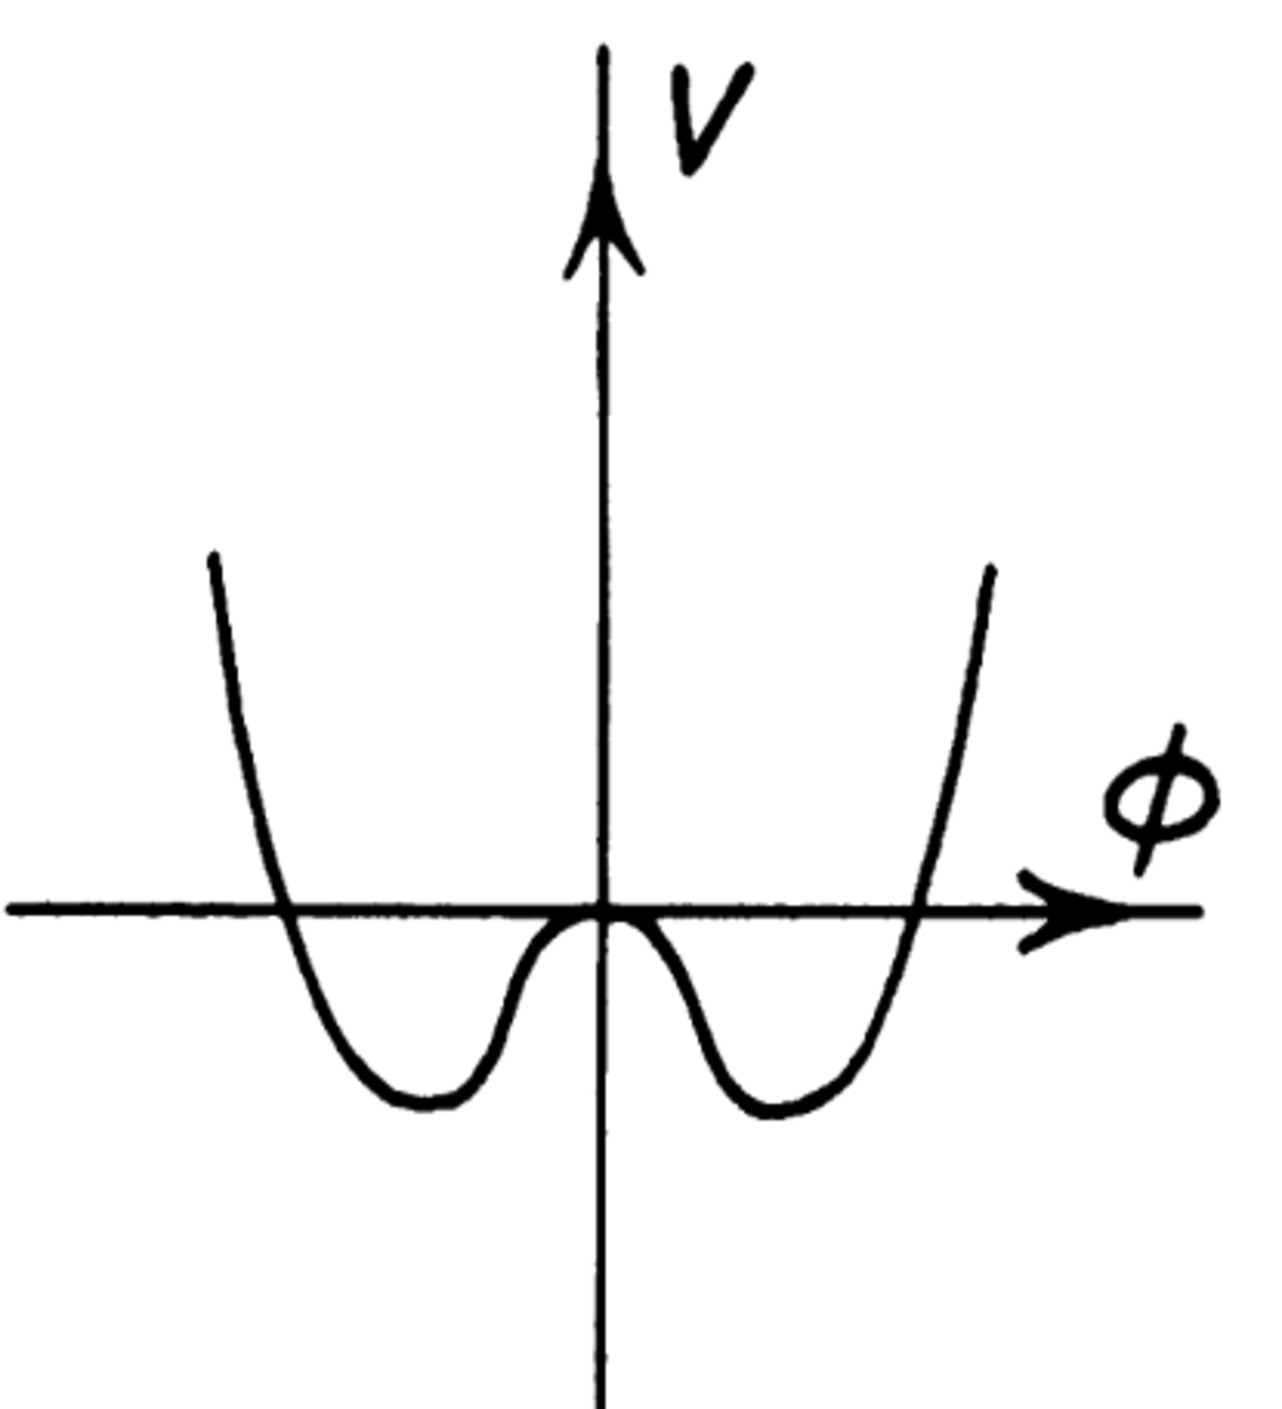
\includegraphics[height=6cm,angle=0]{IMAGEN1.pdf}
\caption{Energ'ia Potencial versus $\phi$.}
\label{fig:1}
\end{figure}
Tenemos
\begin{equation}\label{ecuacion8.4}
\phi=\pm\sqrt{\frac{-\mu^{2}}{\lambda}}\equiv v,
\end{equation}
los cuales son valores distintos de cero para $\phi$ en donde se minimiza el potencial. Luego $\phi$
  toma el valor $v$
  en el estado fundamental, $v$
  es llamado valor de expectaci'on de vac'io de $\phi$.
  El campo $\phi$
  es llamado un campo de Higgs.

Para determinar el espectro de la part'icula, debemos estudiar la teor'ia en la regi'on del m'inimo, entonces hacemos
\begin{equation}\label{ecuacion8.5}
\phi(x)=v+\eta(x),
\end{equation}
luego estamos expandiendo alrededor de $\eta=0$.
  Notemos que de igual manera pudimos haber elegido $\phi=-v+\eta(x)$,
  pero las conclusiones f'isicas son independientes de esta elecci'on, puesto que dijimos que la teor'ia es sim'etrica bajo $\phi\rightarrow-\phi$.
  Substituyendo \eqref{ecuacion8.5} en $\mathcal{L}$
  tenemos
\begin{equation}
\begin{aligned}
\mathcal{L}&=\frac{1}{2}\left(\partial^{\mu}\eta\partial_{\mu}\eta\right)-\left\{ \frac{1}{2}\mu^{2}\left[v^{2}+2\eta v+\eta^{2}\right]+\frac{1}{4}\lambda\left[v^{4}+4v^{3}\eta+6v^{2}\eta^{2}+4v\eta^{3}+\eta^{4}\right]\right\}\\ &=\frac{1}{2}\left(\partial^{\mu}\eta\partial_{\mu}\eta\right)-\left\{ \frac{v^{2}}{2}\left(\mu^{2}+\frac{1}{2}\lambda v^{2}\right)+\eta v\left(\mu^{2}+\lambda v^{2}\right)+\frac{\eta^{2}}{2}(\mu^{2}+3\lambda v^{2})+\lambda v\eta^{3}+\frac{1}{4}\lambda\eta^{4}\right\} .
\end{aligned}
\end{equation}
Usando \eqref{ecuacion8.4}, el t'ermino lineal en $\eta$
  desaparece (cerca del m'inimo), y $\mathcal{L}$
  se reduce a
\begin{equation}\label{ecuacion8.7}
\mathcal{L}=\frac{1}{2}\left(\partial^{\mu}\eta\partial_{\mu}\eta\right)-\left(\lambda v^{2}\eta^{2}+\lambda v\eta^{3}+\frac{1}{4}\lambda\eta^{4}\right)+\text{cte}.
\end{equation} 
El t'ermino con $\eta^{2}$
  tiene el signo correcto, por lo tanto puede ser interpretado como un t'ermino de masa. Este lagrangiano representa a un part'icula con masa
\begin{equation}
m_{\eta}^{2}=2\lambda v^{2}=-2\mu^{2},
\end{equation}
y con dos interacciones, una c'ubica de fuerza $\lambda v$
  y una a la cuarta de fuerza $\lambda/4$.
  Notemos que ambas dependen de $\lambda$,
  el cual es un par'ametro libre hasta donde sabemos. La constante puede ser despreciada dado que el nivel cero del potencial puede ser redefinido.

Las dos descripciones de la teor'ia, en t'erminos de $\phi$
  o $\eta$,
  debe ser equivalente si el problema es resuelto en forma exacta. Si queremos una descripci'on perturbativa es esencial perturbar alrededor del m'inimo para tener una descripci'on valida (convergente). La part'icula escalar descrita por la teor'ia con $\mu^{2}<0$
  es un escalar real, con una masa obtenida por sus propias interacciones con otros escalares, dado que el m'inimo del potencial no tiene un valor cero para el valor de expectaci'on $v$.
  No hay rastro de la simetr'ia de reflexi'on $\phi\rightarrow-\phi$
  en la ecuaci'on \eqref{ecuacion8.7}. Una memoria de esto es preservado en la interacci'on de t'ermino $\eta^{3}$. Puesto que la simetr'ia est'a quebrada, entonces cuando un vac'io espec'ifico fue elegido, el vac'io no tiene la simetr'ia del lagrangiano original. Cada vez que esto ocurre se llama \textbf{quiebre espont'aneo de simetr'ia}.
\subsection{Campo Escalar Complejo}
Supongamos que $\phi$
  es un escalar complejo 
\begin{equation}
\phi=(\phi_{1}+i\phi_{2})/\sqrt{2},
\end{equation}  
y  
\begin{equation}
\mathcal{L}=(\partial_{\mu}\phi)^{*}(\partial^{\mu}\phi)-\mu^{2}\phi^{*}\phi-\lambda(\phi^{*}\phi)^{2}.
\end{equation}
Este es invariante bajo una transformaci'on de gauge global,
\begin{equation}
\phi\rightarrow\phi^{\prime}=e^{i\chi}\phi,
\end{equation}
entonces la simetr'ia de $\mathcal{L}$
  es ahora una simetr'ia global $U(1)$
  en lugar de una reflexi'on como en el ejemplo de \ref{subseccion1} . Escribiendo en t'erminos de las componentes,
  \begin{equation}\label{ecuacion8.11}
  \mathcal{L}=\frac{1}{2}(\partial_{\mu}\phi_{1})^{2}+\frac{1}{2}(\partial_{\mu}\phi_{2})^{2}-\frac{1}{2}\mu^{2}(\phi_{1}^{2}+\phi_{2}^{2})-\frac{\lambda}{4}(\phi_{1}^{2}+\phi_{2}^{2})^{2}.
  \end{equation}
  \begin{figure}[H]
 \centering
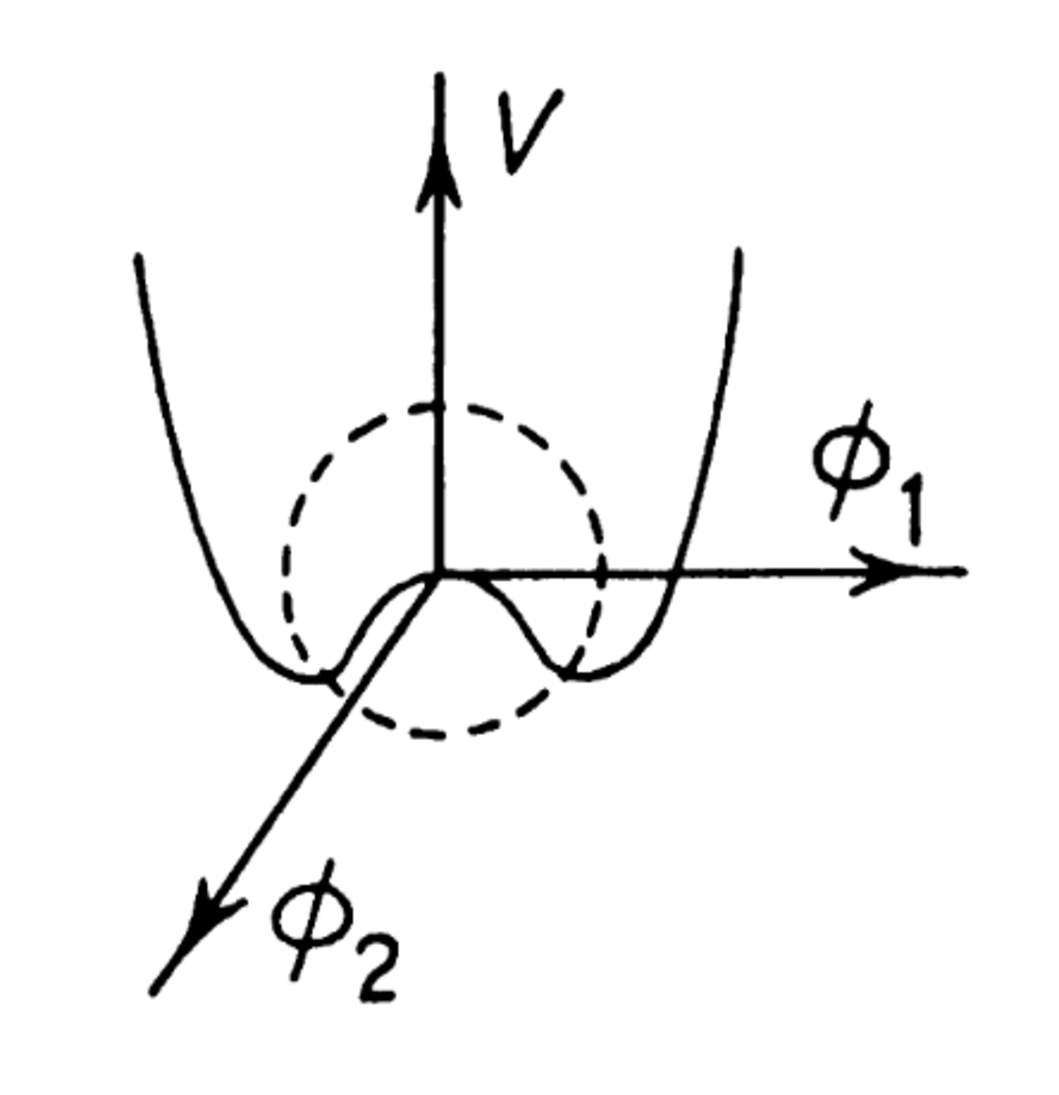
\includegraphics[height=6cm,angle=0]{IMAGEN2.pdf}
\caption{Energ'ia Potencial en funci'on de $\phi_{1}$ y $\phi_{2}$.}
\label{fig:2}
\end{figure}
 En el plano $\phi_{1},\,\phi_{2}$
  (figura \eqref{fig:2}), la energ'ia potencial es claramente un m'inimo en el origen si $\mu^{2}>0$,
  y para $\mu^{2}<0$
  el m'inimo es un circulo de radio 
\begin{equation}
\phi_{1}^{2}+\phi_{2}^{2}=\frac{-\mu^{2}}{\lambda}=v^{2}.
\end{equation}
Para analizar el caso con $\mu^{2}<0$
  tenemos que expandir cerca de $\phi_{1}^{2}+\phi_{2}^{2}=v^{2}$.
  Podemos elegir cualquier punto sobre el circulo, pero debemos elegir alg'un punto, el cual rompera la simetr'ia para la soluci'on. Escogemos, arbitrariamente, el punto $\phi_{1}=v,\,\phi_{2}=0$,
  y escribimos, con $\eta$
  y $\rho$
  reales,
  \begin{equation}
  \phi=\frac{v+\eta(x)+i\rho(x)}{\sqrt{2}}.
  \end{equation}
  Substituyendo en \eqref{ecuacion8.11}, encontramos un lagrangiano que puede ser interpretado en t'erminos de part'iculas y sus interacciones:
\begin{equation}\label{ecuacion8.14}
\mathcal{L}=\frac{1}{2}(\partial_{\mu}\rho)^{2}+\frac{1}{2}(\partial_{\mu}\eta)^{2}+\mu^{2}\eta^{2}-\lambda v\left(\eta\rho^{2}+\eta^{3}\right)-\frac{\lambda}{2}\eta^{2}\rho^{2}-\frac{\lambda}{4}\eta^{4}-\frac{\lambda}{4}\rho^{4}+\text{cte}.
\end{equation}
Los primeros t'erminos corresponden a la energ'ia cin'etica. El t'ermino $+\mu^{2}\eta^{2}$
  nos dice que el campo $\eta$
  corresponde a una part'icula de masa $m_{\eta}^{2}=2\left|\mu^{2}\right|$.
  El t'ermino en $\rho^{2}$
  a desaparecido, implicando que el campo $\rho$
  no tiene masa. Este es llamado bos'on de Goldstone. Existe un teorema general que dice, cualquiera sea una simetr'ia global continua que  est'a espontaneamente rota, el espectro contendr'a un boson de esp'in cero sin masa (bos'on de Goldstone).

T'ecnicamente es claro como el bos'on sin masa aparece. El potencial es un m'inimo a lo largo de un c'irculo. Excitaciones en la direcci'on radial requieren  tirar el potencial fuera del m'inimo y una masa est'a asociada con la curvatura del potencial. A lo largo del c'irculo el potencial es plano, entonces no hay resistencia al movimiento alrededor del c'irculo, lo cual es el resultado de la excitaci'on sin masa. La simetr'ia $U(1)$
  es rota dado la necesidad de elegir un punto en particular sobre el c'irculo sobre el cual se expande. La presencia y particular forma de los t'erminos de interacci'on en \eqref{ecuacion8.14} proveen una memoria de la simetr'ia, pero no de una forma obvia.
\section{Mecanismo de Higgs}
\subsection{Caso Abeliano}
Previamente consideramos una invariancia global de gauge. Ahora consideremos una local, hagamos el lagrangiano invariante bajo una transformaci'on local de gauge. Sabemos que la invariancia bajo una tranformacion local de gauge requiere la introducci'on de un campos $A_{\mu}$
  sin masa, y debemos escribir el lagrangiano en t'erminos de la derivada covariante. Entonces
\begin{equation}
\partial_{\mu}\rightarrow D_{\mu}=\partial_{\mu}-igA_{\mu}.
\end{equation}
El campo de gauge transforma como
\begin{equation}
A_{\mu}\rightarrow A_{\mu}^{\prime}=A_{\mu}-\frac{1}{g}\partial_{\mu}\chi(x)
\end{equation}
y $\phi$ es invariante bajo
\begin{equation}\label{ecuacion8.17}
\phi(x)\rightarrow\phi^{\prime}(x)=e^{i\chi(x)}\phi(x).
\end{equation}
As'i el lagrangiano es
\begin{equation}\label{ecuacion8.18}
\mathcal{L}=(D_{\mu}\phi)^{*}(D_{\mu}\phi)-\mu^{2}\phi^{*}\phi-\lambda(\phi^{*}\phi)^{2}-\frac{1}{4}F_{\mu\nu}F^{\mu\nu}.
\end{equation}
Para $\mu^{2}>0$
  este describe la interacci'on de una part'icula escalar cargada (con $g\equiv e$)
  de masa $\mu$
  con el campo electromagn'etico $A_{\mu}$,
  por ejemplo. Notemos que no hay un t'ermino de masa para $A_{\mu}$.
  Queremos elegir $\mu^{2}<0$
  como en las secciones anteriores. Notemos que el lagrangiano contiene cuatro campos independientes o grados de libertad, los dos campos escalares $\phi_{1}$
  y $\phi_{2}$, y los dos estados de polarizaci'on transversal del bos'on sin masa. 

La ecuaci'on \eqref{ecuacion8.17} nos dice que la teor'ia ser'a invariante bajo una transformaci'on de gauge de $\phi(x)$.
  En general $\phi$ puede ser escrito de la forma
  \begin{equation}
  \phi(x)=\eta(x)e^{-i\rho(x)}
  \end{equation}
  donde $\eta,\,\rho$
  son reales, por lo que podemos reescribir $\phi(x)$
  de la forma
  \begin{equation}
  \phi(x)=\frac{v+h(x)}{\sqrt{2}}
  \end{equation}
  con $h$
  real, habiendo usado una transformaci'on como $\phi\rightarrow e^{i\chi(x)}\phi$.
  Substituyendo en $\mathcal{L}$ tenemos
  \begin{equation}
  \begin{aligned}
  \mathcal{L}&=\frac{1}{2}[(\partial^{\mu}+igA^{\mu})(v+h)][(\partial_{\mu}-igA_{\mu})(v+h)]-\frac{\mu^{2}}{2}(v+h)^{2}-\frac{\lambda}{4}(v+h)^{4}-\frac{1}{4}F_{\mu\nu}F^{\mu\nu}\\
  &=\frac{1}{2}(\partial_{\mu}h)(\partial^{\mu}h)+\frac{1}{2}g^{2}v^{2}A_{\mu}A^{\mu}-\lambda v^{2}h^{2}-\lambda vh^{3}-\frac{\lambda}{4}h^{4}+g^{2}vhA^{\mu}A_{\mu}+\frac{1}{2}g^{2}h^{2}A_{\mu}A^{\mu}-\frac{1}{4}F_{\mu\nu}F^{\mu\nu}.
  \end{aligned}
  \end{equation}
  Aqu'i cada t'ermino puede ser interpretado. Hay un resultado interesante, ahora hay un t'ermino de masa para el bos'on de gauge!. Pero dado que comenzamos con una teor'ia invariante de gauge e hicimos solo transformaciones algebr'aicas, esperamos que la teor'ia resultante sea invariante de gauge tambi'en. La masa del bos'on de gauge es la raiz cuadrada del coeficiente de $A_{\mu}A^{\mu}/2$,
  \begin{equation}
  M_{A}=gv,
  \end{equation}
 y este es distinto de cero solo cuando la simetr'ia de gauge esta espont'aneamente quebrada por el campo de Higgs adquiriendo un valor de expectaci'on de vac'io. Entonces la teor'ia es solo invariante de gauge en un sentido restringido. El lagrangiano es invariante de gauge pero el vac'io no lo es, porque hemos escogido una direcci'on particular en $\phi_{1},\,\phi_{2}$ para el potencial m'inimo.
 El espectro es ahora un unico boson de Higgs real $h$,
  con masa $\sqrt{(2\lambda v^{2})}$, varias interacciones propias e interacciones c'ubicas y cuarticas con el campo de gauge $A_{\mu}$,
  m'as un bos'on $A_{\mu}$.
  Dado que el bos'on masivo tiene 3 estados de spin ( correspondientes a $J_{z}=1,\,0,\,-1$)
  el n'umero de campos independientes es a'un cuatro, lo que es consistente.

Lo que ha ocurrido aqu'i es que el bos'on de Goldstone de la secci'on anterior se ha convertido en el estado de polarizaci'on longitudinal del bos'on de gauge. 'Este fen'omeno se le refiere a veces diciendo que el bos'on de gauge se \textit{come} al bos'on de Goldstone. El mecanismo anterior es llamado como \textbf{Mecanismo de Higgs}.